%!TEX root = ../document.tex
\chapter{Project Risk Management}

During project implementation, there will be inevitably some problems and risks. It's very important to summary timely, consider seriously, coordinate correctly and make the right decision.

Our budget is about 200 millions dollar at the beginning. We plan to cooperate with the government and some other companies later. As a result, we have a very strong risk tolerance. Trying to promote the development of the flying car, we prefer using the new technologies such as composite materials, AI. Though this preference will cause more risks.

To identify the risks, we used the brainstorm, interview and research methods. But the SWOT analyse method was mainly used. 

\section{SWOT analysis}

\subsection{Strength}

\begin{itemize}
\item We have a enough budget to support the project as mentioned at the beginning of this chapter,. This will become our very important key. 
\item There are many mature and advanced design, technologies to apply as the technological development is changing with each passing day. We can have more options to solve the problems.
\item We have many experienced engineers and designers from the field of automobile and the domain of the aircraft.
\item Nowadays, people buy more and more cars, which makes the traffic jams worse. According to the market analyst, the the flying car is prospective in 20 years. 
\end{itemize}

\subsection{Weakness}

\begin{itemize}
\item Our company don’t have any experience of designing a flying car before, which requires our two domain engineers and designers work together.
\item Our company is short of the professional airworthiness personnel who has the ability of  transforming the regulations of the airworthiness certification to the detail technical criteria.
\end{itemize}

\subsection{Opportunity}

\begin{itemize}
\item Make a breakthrough to our company in the flying car design.
\item Other flying car companies give us technical or kind of supports.
\item Become a leader in the flying car market by using the new technology.
\end{itemize}

\subsection{Threat}

\begin{itemize}
\item Similar companies raise certification standards and cause project failure.
\item Meet many pressures from the other same kind of companies when our products come into market.
\item The project that involves in many departments makes the management complicated.
\item There are some other unstable and unknown factors will threat our project like the financial crisis.
\end{itemize}

\section{Main risks}

By using different risks analyse methods, we conclude that the primary risks can be divided into the main risks and some additional risks for the Flying Car project. Their risk score is obtained by the risk matrix table attached at the end of this chapter. The main risks generally include the following four parts:

\subsection{Technology and design risks}

The Flying Car need to fly and have the ability of collision. As a result, it have to balance the relation between the weight and the strength, which takes more challenges to our engineers and designers. These challenges will bring more risks to the project compared to the traditional car project. The project may be failed due to the technology and design challenges. It’s risk score is 1.
\begin{enumerate}
\item Use some advance technologies and materials to overcome the challenges.

\item Optimize the load factor on the body to decrease the material request. 

\item Use some special structure design to balance the weight and the strength.
\end{enumerate}

\subsection{Certification risk}

Our project Flying Car must obtain two certifications: the certification of the car and the certification of airworthiness. The certification will last for a long time especially the certification of airworthiness, the long-time certification procedure may block our project progress.

Something worse is that the structure or some systems need to be redesigned and then may restart the certification of the airworthiness. This risk will block the project progress seriously. The certification risk score is 1.

\begin{enumerate}
\item Make a clear design-certification-production timetable.

\item Store the technological documents for the future certifications.

\item Use the simulator to test and verify the product for the certifications.

\item Engineers and designers should think twice and verify the characteristics before handling on the final product.

\item Refer to the design and solutions of other similar products.
\end{enumerate}

\subsection{Market risk}

As a new kind of transportation, we can not assure our Flying Car market and whether the customers accept the product. It’s a risk that our product may not be very popular and the sells can’t meet our expectation.There is a big risk that our Flying Car may won’t have the available airspace. The market risk score is 5.

\begin{enumerate}
\item Cooperate with the government to apply for the airspace.

\item Propose a flying car management method.

\item Make some advertisements on TV, radio and the Internet.

\item Organize some test activities to show our Flying Car’s safety and efficiency.
\end{enumerate}

\subsection{Budget risk}

Firstly, the usage of the advance technologies and materials like the aluminum alloy and the titanium alloy will require a big expense; Secondly, the certification of the airworthiness requires several fly tests. The fly test and the redesign will cost a lot and bring some useless expenses; Thirdly, the advertisements and the organization of the activities will cost a lot of our budget.

It’s very possible that these three factors lead us to run out of out budget and cause the project failed. The budget risk score is 8.

\begin{enumerate}
\item Cooperate with the government to get the financial subsidy.

\item Cooperate with other companies to be financed.

\item Decrease the predefined performance level.

\item Loan to banks.
\end{enumerate}

\section{Additional risks}

There are some additional risks too, which are concerned with the implementation, the production and the management. They are listed as following:

\subsection{Implementation risks}

This project is involved with many departments who may have different implementation situation. It’s very possible that some departments can’t guarantee the progress and that there will be some implementation cycle delays. The implementation cycle delays will interrupt the project. This risk score is 6.

\begin{enumerate}
\item The hole company need to set a unique design-production timeline and apply the manage.

\item Build a clear information transmission and step synchronization at the beginning of the project.

\item Make a clear holiday arrangement at beginning to avoid the risk of the interruption by the holiday like the Christmas.
\end{enumerate}

\subsection{Production risks}

To product a flying car, there are many manufactures to cooperate with each other. And these manufactures may come from different regions and different countries. So it will be a big problem to synchronize these manufactures and to guarantee their tasks. We may cause some misunderstands due to the different languages and different cultures. The production risks will block our flying car production procedure. This risk score is 7.

\begin{enumerate}
\item Send a quality checker and a progress monitor to the manufactures. They send back the report to the headquarters frequently.

\item Hire the qualified translator who has the ability of the foreign language, who knows well about the foreign culture and who has the relative diploma.
\end{enumerate}

\subsection{Worker risks}

\begin{enumerate}
\item Worker has a negative response to the project implementation, lacks of passion, idleness, etc. The risk score is 6.

\textbf{Solution:} Establish effective reward and punishment measures and publicize it’s consequences.

\item invalid project organization. The risk score is 9.

\textbf{Solution:} According to the progress of the project, dismiss or reorganize the project organization.

\item Spread rumors and crack down on project implementation team members. The risk score is 10.

\textbf{Solution:} Regularly announce the progress of the project implementation and impose penalties on those who spread the rumors.

\item The middle and senior leaders arranged other affairs to the implementation people, resulting in the implementation progress not being completed on time. The risk score is 6

\textbf{Solution:} If the implementation people need to deal with other matters, he must be approved by the project implementation leadership team.

\item Because after the new process is established, it may affect the interests of relevant personnel, especially the interests of middle and high-level, leading to resistance to the project and ultimately affecting the project implementation process;The risk score is 5.

\textbf{Solution:} Convene a special middle-level and high-level coordination meeting to implement a unified understanding of the Flying Car project, clear goals, and coordinate their interests by the top leadership.
\end{enumerate}

\subsection{Management risks}

\begin{enumerate}
\item The departments meet conflicts during the application process. The risk score is 6.

\textbf{Solution:} Senior leaders give arbitration from the overall interests of the company.

\item For the personal benefit, the business processing is performed without authorization. The risk score is 5.

\textbf{Solution:} The executives of each implementing unit must obtain the authorization.

\item The senior management should stand at the height of overall optimization at a critical moment and conduct arbitration. The risk score is 10.
\end{enumerate}

The following page shows the risk matrix of the program.

\begin{figure}[!htb]
\centering
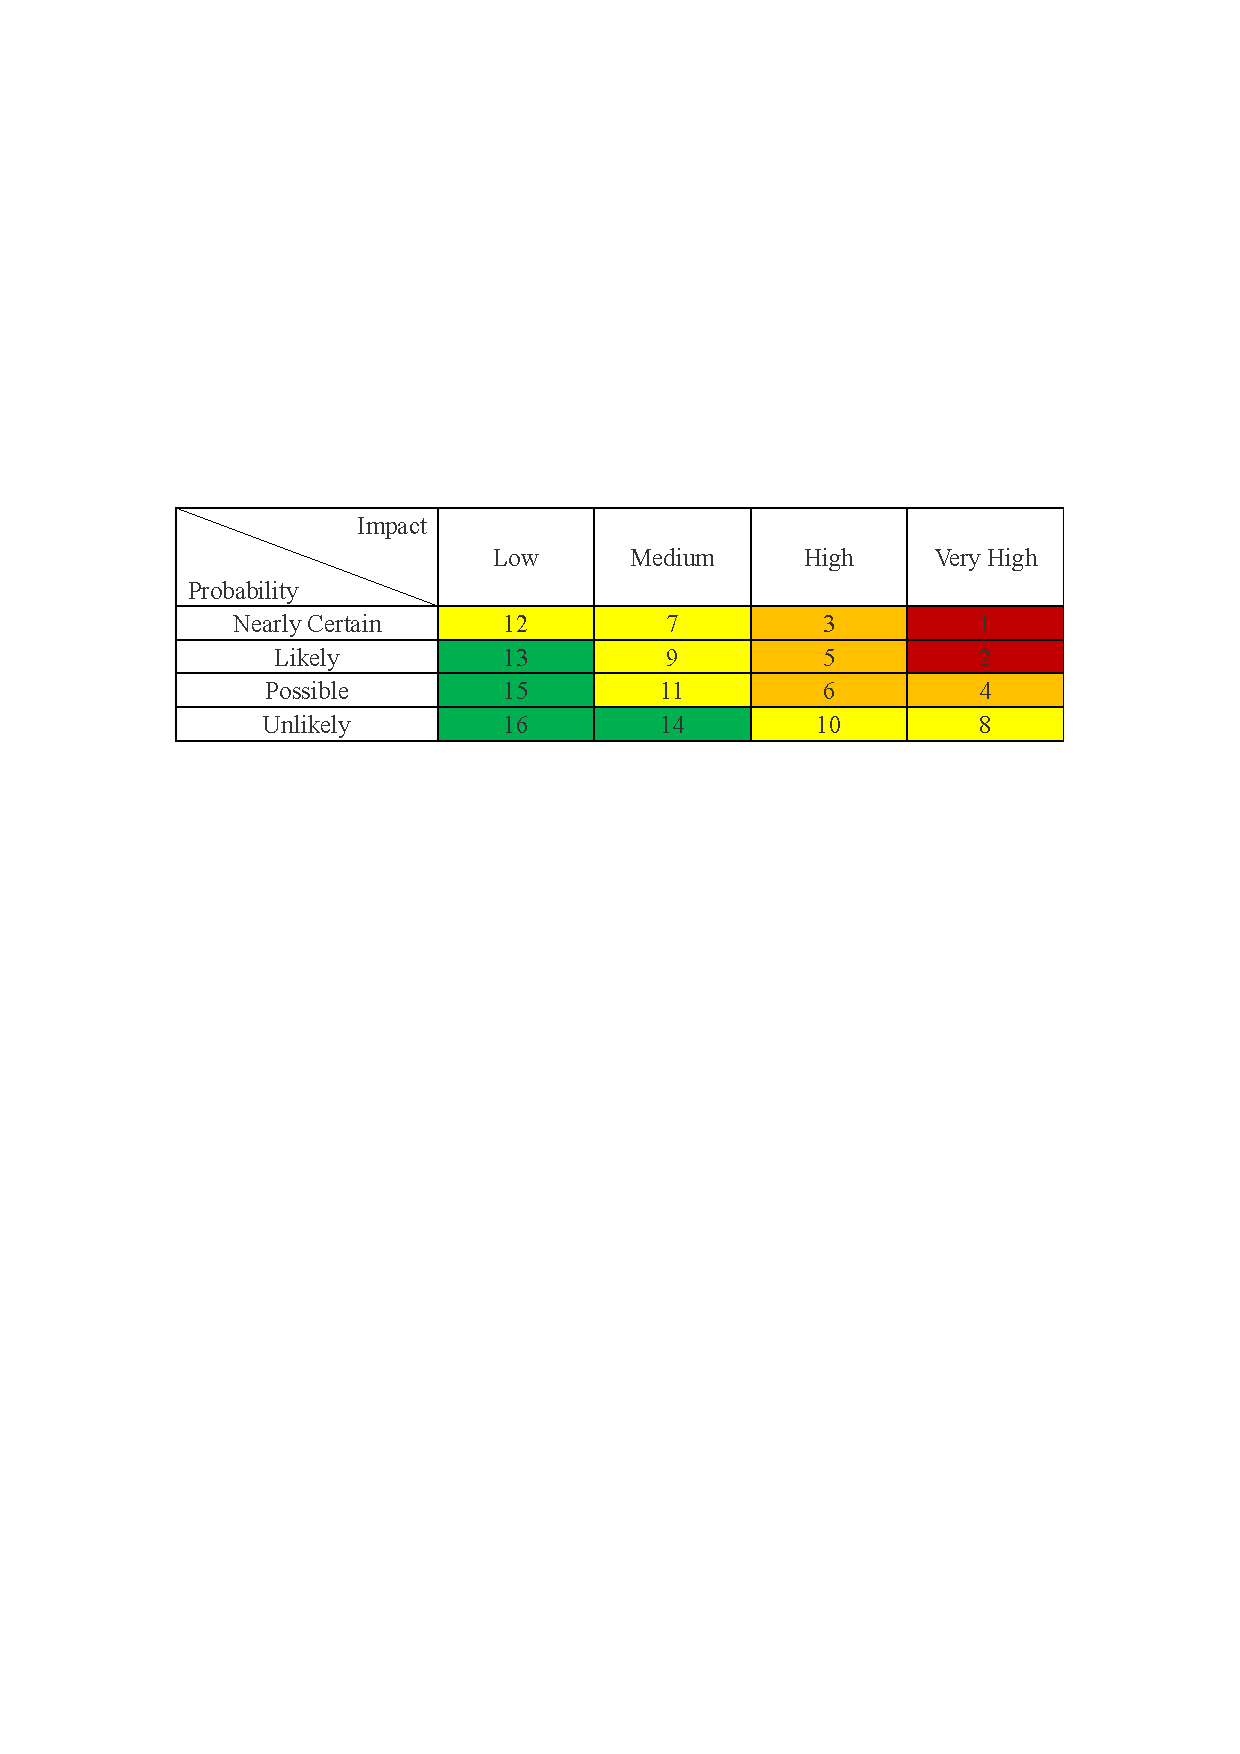
\includegraphics[width=15cm]{pic/riskMatrix.pdf}
% \caption{单转换超外差接收机\protect\footnotemark}
% \label{fig:dlr_ads-b_receiver}
\end{figure}